\documentclass[fleqn]{article}

\usepackage[utf8x]{inputenc} 
\usepackage[T1]{fontenc}
\usepackage{textcomp}
\usepackage{gensymb}
\usepackage{titling}
\usepackage{lipsum}
\usepackage{url}
\usepackage{graphicx}
\usepackage{color}
\usepackage[usenames,dvipsnames,svgnames,table]{xcolor}
\usepackage{amsmath}
\usepackage{amsmath}
\usepackage{amsthm}
\usepackage{amssymb}
\graphicspath{{images/}}

\title{Trabalho Extra}

\author{Pedro Delfino}

\begin{document}

\maketitle

\newpage

\section*{Primeira Questão [AS, exercício 3]} 

\paragraph{Sejam $a,b,c,r$ constantes reais com $r \neq 0$, e considere a curva \\ $\gamma: \mathbb{R}  \rightarrow \mathbb{R}^3 $ definida por:}

\begin{center}
$\gamma(t) = (r\cos t,r\sin t, a\sin t + b\cos t +c) $ 
\end{center}

\paragraph{a) Prove que a curva é plana.}
\paragraph{b) Determine se é uma curva circular, isto é, se ela coincide com o arco de uma circuferência. \\} 

\begin{proof}
  \begin{align*}
  &  \text{Seja: } \gamma(t) =  (r \cos t,r\sin t, a\sin t + b\cos t +c)  \\
   & \text{Primeira derivada: }\gamma'(t) = (-r\sin t,r\cos t,   a\cos t - b\sin t)  \\
   & \text{Segunda derivada: }\gamma''(t) = (-r\cos t,-r\sin t,    -a\sin t - b\cos t)  \\
   & \text{Terceira derivada: }\gamma'''(t) = (r\sin t,-r\cos t, -a\cos t + b\sin t)  \\
   & \text{A torção pode ser expressa por: }\tau  = {{\left(   {r' \times r''} \right) \cdot r'''} \over {\left\| {r' \times r''} \right\|^2}}\\
   & \text{A fórmula acima não exige que a curva esteja      parametrizada pelo cumprimento   de arco} \\
   & \text{Desenvolvendo os cálculos do numerador}  \\
   & \text{O produto vetorial das duas primeiras derivadas é:  } {\gamma'(t) \times \gamma''(t)= (-rb, -  ra, r²)}\\
   & \text{O produto escalar é o produto vetorial vezes a   terceira derivada: } \\
   & (-rb, -ra, r²)\cdot \gamma'''(t)  \\
   & (-rb, -ra, r²)\cdot (r\sin t,-r\cos t, -a\cos t + b\sin t)   = 0 \\
   & \text{O numerador é zero. Logo, a torção é zero. } \\
   & \tau = 0 \\
   & \text{Se a torção é zero, a curva é plana.} 
  \end{align*}
\end{proof}


\begin{proof}
\begin{align*}
  & \text{A curvatura pode ser expressa por: }\kappa = \frac{\|\gamma' \times \gamma''\|}{\|\gamma'\|^3}\\
  & \text{A fórmula acima não exige que a curva esteja  parametrizada pelo cumprimento   de arco} \\
  & \text{A curvatura constante indica que a curva é circular} \\
  & \text{O produto vetorial das duas primeiras derivadas é:  }{\gamma'(t) \times \gamma''(t)= (-rb, -  ra, r²)}\\ 
  & \text{O módulo do produto vetorial: } ||\gamma' \times \gamma''\| = \sqrt{r^2b^2+r^2a^2+r^4}  \\
  & \text{Como pode ser visto, o numerador só envolve constantes} \\
  &\text{O denominador, por sua vez, é: } ||\gamma'| |^3 \\
  & ||\gamma'\|^3 = (\sqrt{r^2+a^2 \cos ^2 t + b^2 \sin ^2 t - ab2 \cos t \sin t })^3 \\
  & \text{O denominador não é constante, estando em função de t. Portanto, } \gamma (t) \text{ não é uma curva circular}
\end{align*}
\end{proof}

Preview:
\bigskip

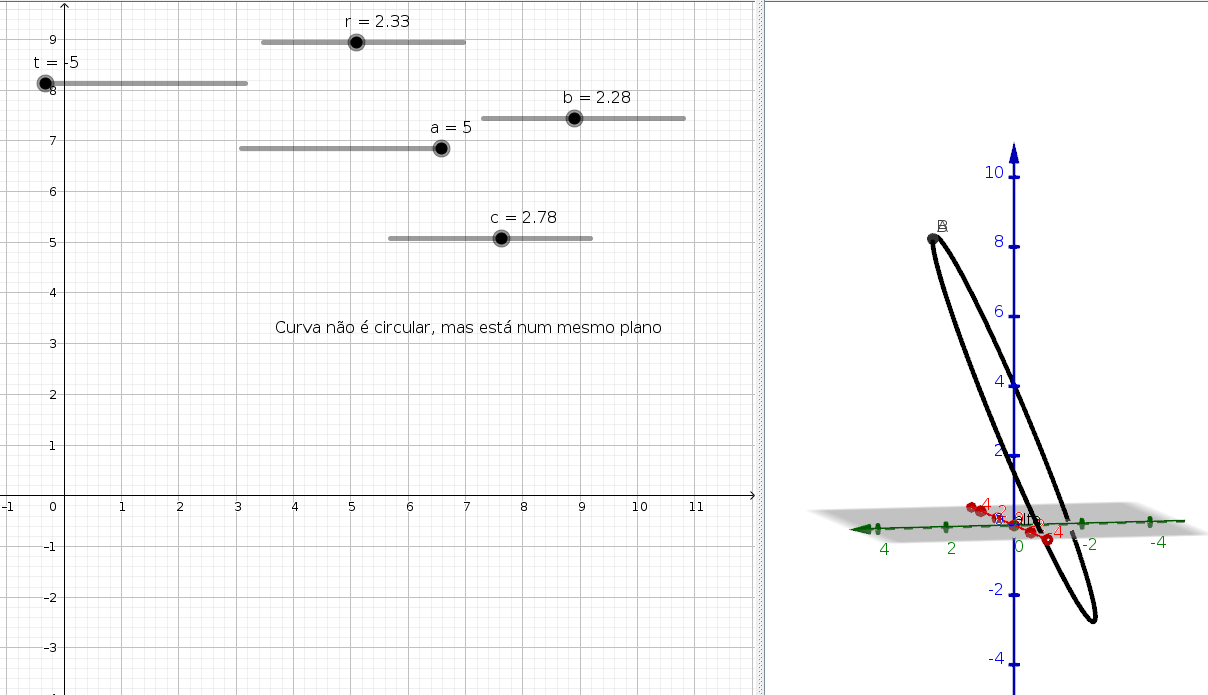
\includegraphics[scale=0.2]{questao-torcao-zero}
\bigskip

\paragraph{Simulação no geogebra disponível em https://github.com/pdelfino/differential-geometry/tree/master/extra-hw}


\newpage

\section*{Segunda Questão [Lista 5, exercício 4]} 

\paragraph{Provar que a interseção de uma quantidade finita de abertos é um conjunto aberto.}

\begin{proof}
\begin{align*}
 & \text{Seja } \Lambda \text{ uma família muito grande de conjuntos abertos u} \\ 
  &\Lambda = \{ u_{1}, u_{2}, u_{3}, ... , u_{\lambda} \} \\
  & \text{Seja x um ponto na interseção de todos esse conjuntos abertos} \\
  &x \in u_{1}, u_{2}, u_{3}, ... , u_{\lambda } \\
  &\text{Como todos os conjuntos } u_{\lambda} \text{ são abertos, existem valores:} \\
  &r_{1}, r_{2}, r_{3}, ... , r_{\lambda } > 0 \\
  &\text{De modo que } \\
 & B(x, r_{1}) \subseteq u_{1},   
   B(x, r_{2}) \subseteq u_{2}, ..., 
    B(x, r_{\lambda}) \subseteq u_{\lambda}  \\
 & \text{Seja } \varepsilon \text{ um número pequeno, maior que zero e definido pela função mínimo}\\
  &\varepsilon = min \{r_{1}, r_{2}, r_{3}, ... , r_{\lambda } \} \\
  &\text{Assim, existe uma bola aberta contida na interseção: } \\
  &   B(x, \varepsilon) \subseteq  \bigcap^\lambda_{i=1} u_{i}  \\
 & \text{Portanto, a interseção de uma quantidade finita de conjuntos abertos é um conjunto aberto.}
\end{align*}
\end{proof}

\bigskip

Essa questão não exige simulação no geogebra.

\newpage

\section*{Terceira Questão [Lista 1, exercício 12]} 


\paragraph{Seja $\alpha (t)$ uma curva regular que não passa pela origem. Se $\alpha (t_{0})$ é o ponto do traço de $\alpha$ mais próximo da origem, mostre que o vetor posição $\alpha (t_{0})$ é ortogonal a $\alpha'(t_{0})$}

\begin{proof}
\begin{align*}
 & \text{Seja } \alpha: I \rightarrow \mathbb{R}  \text{ uma curva regular que não passa pela origem} \\
  & \alpha (t_{0}): \text{o ponto do traço de } \alpha  \text{ mais próximo da origem}\\
&   \text{Se } \alpha (t_{0}) \perp \alpha'(t_{0}) \\
 &  \text{Então } \alpha (t_{0}) \cdotp \alpha'(t_{0}) = 0 \\
 & \text{A função } t \rightarrow  || \alpha (t) ||^2 \text{ tem um mínimo em }  t_{0}    \\
&  \text{Logo, } t_{0} \text{ é um ponto crítico, isto é } \\
 & \dfrac{d}{dt} |_{t = t_{0}} \quad  \quad  || \alpha (t) ||^2 = 0 \\
  &\text{Então, } 2\alpha'(t_{0})\alpha (t_{0})=0   \\ 
  &\alpha'(t_{0})\alpha (t_{0})=0
\end{align*}
\end{proof}

\bigskip

Essa questão não exige simulação no geogebra.

\newpage

\section*{Quarta Questão [Lista 3, exercício 7]} 

\paragraph{Demonstrar que a curva ${\alpha (t) =  (t, \frac{1+t}{t}, \frac{1-t^2}{t})}$  está incluída num plano} 

\begin{proof}
\begin{align*}
 & \text{Seja a equação geral do plano definida por:} \\
 & a(x) + b(y) + c(z) = d \\
 & \text{Inserido os parâmetros:} \\
 & a(t) + b(\frac{1+t}{t}) + c(\frac{1-t^2}{t}) = d \\    
 & a(t^2) + b(1+t) + c(1-t^2) = d(t) \\
 & \text{Reorganizando:} \\
 & t^2(a-c)+t(b-d)+(b+c)=0 \\
 & \text{Para essa igualdade ser verdadeira é preciso que:}  \\
 & a - c = 0 \\
 & b - d = 0 \\
 & b + c = 0 \\
 & \text{Os coeficientes podem ficar em função de "a"}\\
 & a = c = - b = - d \\
 & a(x) + b(y) + c(z) = d \\
 & a(x) + (-a)(y) + (a)(z) = (-a)\\
 & \text{Dividindo tudo por "a"}\\
 & 1x -1y +1z = -1\\
\end{align*}
\end{proof}

\bigskip

O vetor normal que define o plano em que esta curva está inserida é (1,-1,1)
  
\newpage

Preview:

\bigskip


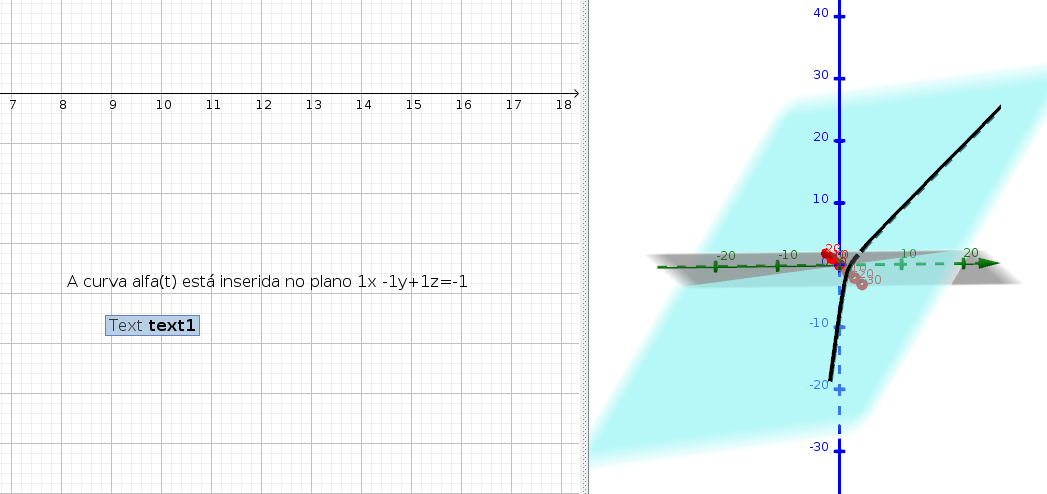
\includegraphics[scale=0.2]{curva-no-plano}

\bigskip

\paragraph{Simulação no geogebra disponível em https://github.com/pdelfino/differential-geometry/tree/master/extra-hw}

\newpage

\section*{Quinta Questão [Lista 4, exercício 13]} 

\paragraph{Provar que a evoluta da elipse $\gamma (t)  = (a \cos t, b \sin t)$  com $ a, b > 0 $ é a astróide:}

$\rho (t) = (\frac{(a^2-b^2) \cos ^3 t}{a},\frac{(b^2-a^2) \sin ^3 t}{b} )$ 

\paragraph{Observação: Considerar que mesmo quando $\beta$ não é parametrizada pelo comprimento de arco, $\alpha$(t)=$\beta$(t)+$\frac{n(t)}{\kappa}$ é a evoluta de $\beta$.}

\begin{proof}
\begin{align*}
&\text{Seja a curvatura de $\rho$:} \\
&\kappa=\frac{ab}{(a^2sen ^2 t+b^2cos ^2 t)^{\frac{3}{2}}}\neq 0 \\
&\text{Seja o vetor normal:} \\ 
&n(t)=\frac{(-bcos t,-asen t)}{(a^2sen^2 t+b^2cos^2 t)^{\frac{1}{2}}} \\
&\text{Assim, } \beta(t)  \\
&\beta(t)=(acos t, bsen t)+\frac{a^2sen^2 t+b^2cos^2 t}{ab}(-bcos t,-asen t) \\
&\beta(t)= (\frac{(a^2-b^2)cos^3 t}{a},\frac{(b^2-a^2)sin^3 t}{b} ) \\
&\text{Há de ser ressaltado que o traço da evoluta é descrito pela astroide:} \\
&(ax)^\frac{2}{3}+(by)^\frac{2}{3}=(a^2-b^2)^\frac{2}{3} \\
&\beta(t) \text{ não é regular nos pontos para os seguintes valores de t} \\
&t=0=\frac{\pi}{2}=\frac{3\pi}{2}
\end{align*}
\end{proof}

\newpage

Preview:
\bigskip

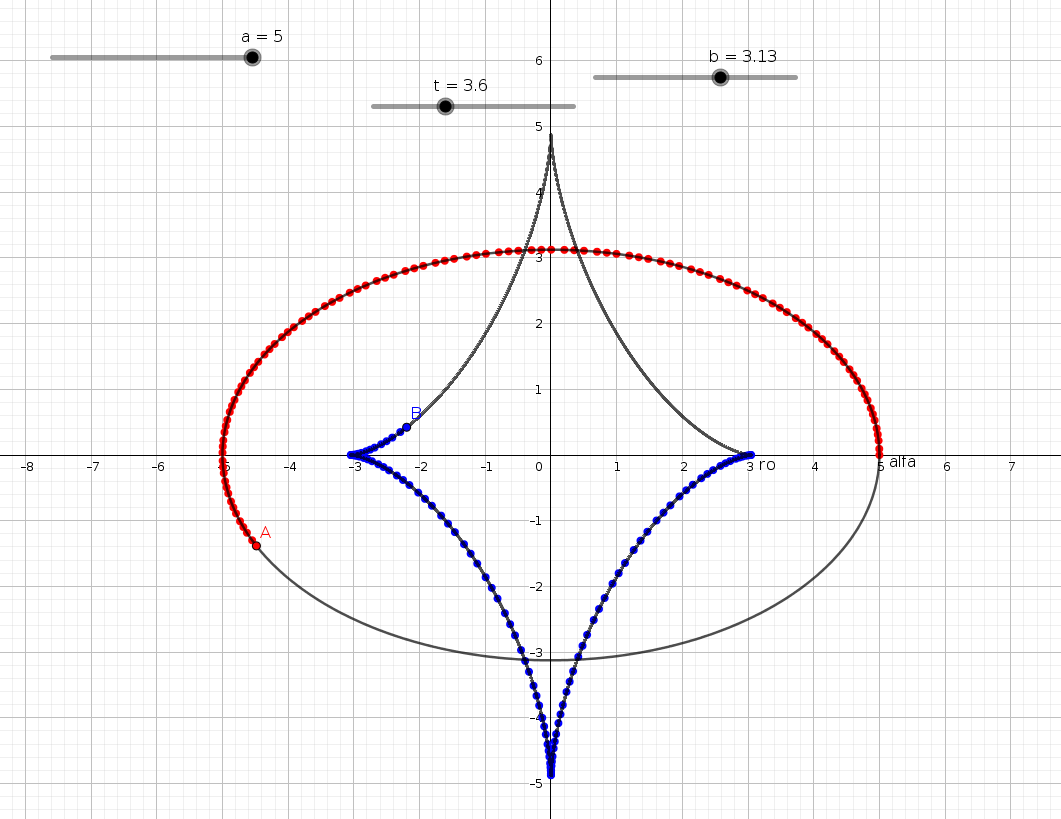
\includegraphics[scale=0.2]{evoluta}
\bigskip

\paragraph{Simulação no geogebra disponível em https://github.com/pdelfino/differential-geometry/tree/master/extra-hw}

\newpage

\section*{Sexta Questão [Lista 8, exercício 3]} 

\paragraph{Mostre que a quádrica $x^2 + 2y^2 + 6x - 4y+ 3z = 7$ é uma superfície, exibindo um atlas.}


\begin{proof}
\begin{align*}
 & S = \{(x,y,z)\in \mathbb{R} / x^2 + 2y^2 + 6x -   4y+ 3z -7 =0 \}\\
 & \text{Assim: } f^{-1}(0)=S  \\
 & \nabla f= (\frac{\partial f}{\partial x},    \frac{\partial f}{\partial y},\frac{\partial f}  {\partial z}) \\
&  \nabla f= (2x+6, 4y - 4, 3) \\
 & \text{Assim: } \\
 & \forall (x,y,z)\in \mathbb{R}  \\
 & \nabla f \neq (0,0,0)\\
 & \text{Logo, pelo teorema das superíficies de  nível, S é uma superfície regular } \\
 & \text{Atlas  } \sigma : (x,y) \rightarrow (x,y,-\frac{x^2}{3}   -\frac{2y^2}{3} -2x + \frac{4}{3}y +\frac{7}{3})
\end{align*}
\end{proof}

Preview:
\bigskip

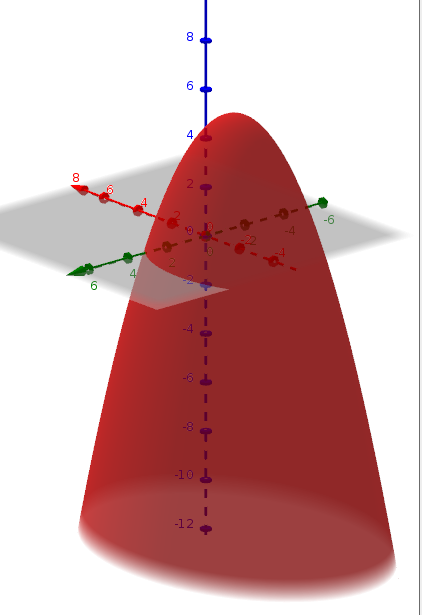
\includegraphics[scale=0.2]{surface}  

\bigskip

\paragraph{Simulação no geogebra disponível em https://github.com/pdelfino/differential-geometry/tree/master/extra-hw}

\end{document} 